\begin{figure}[!t]
\centering
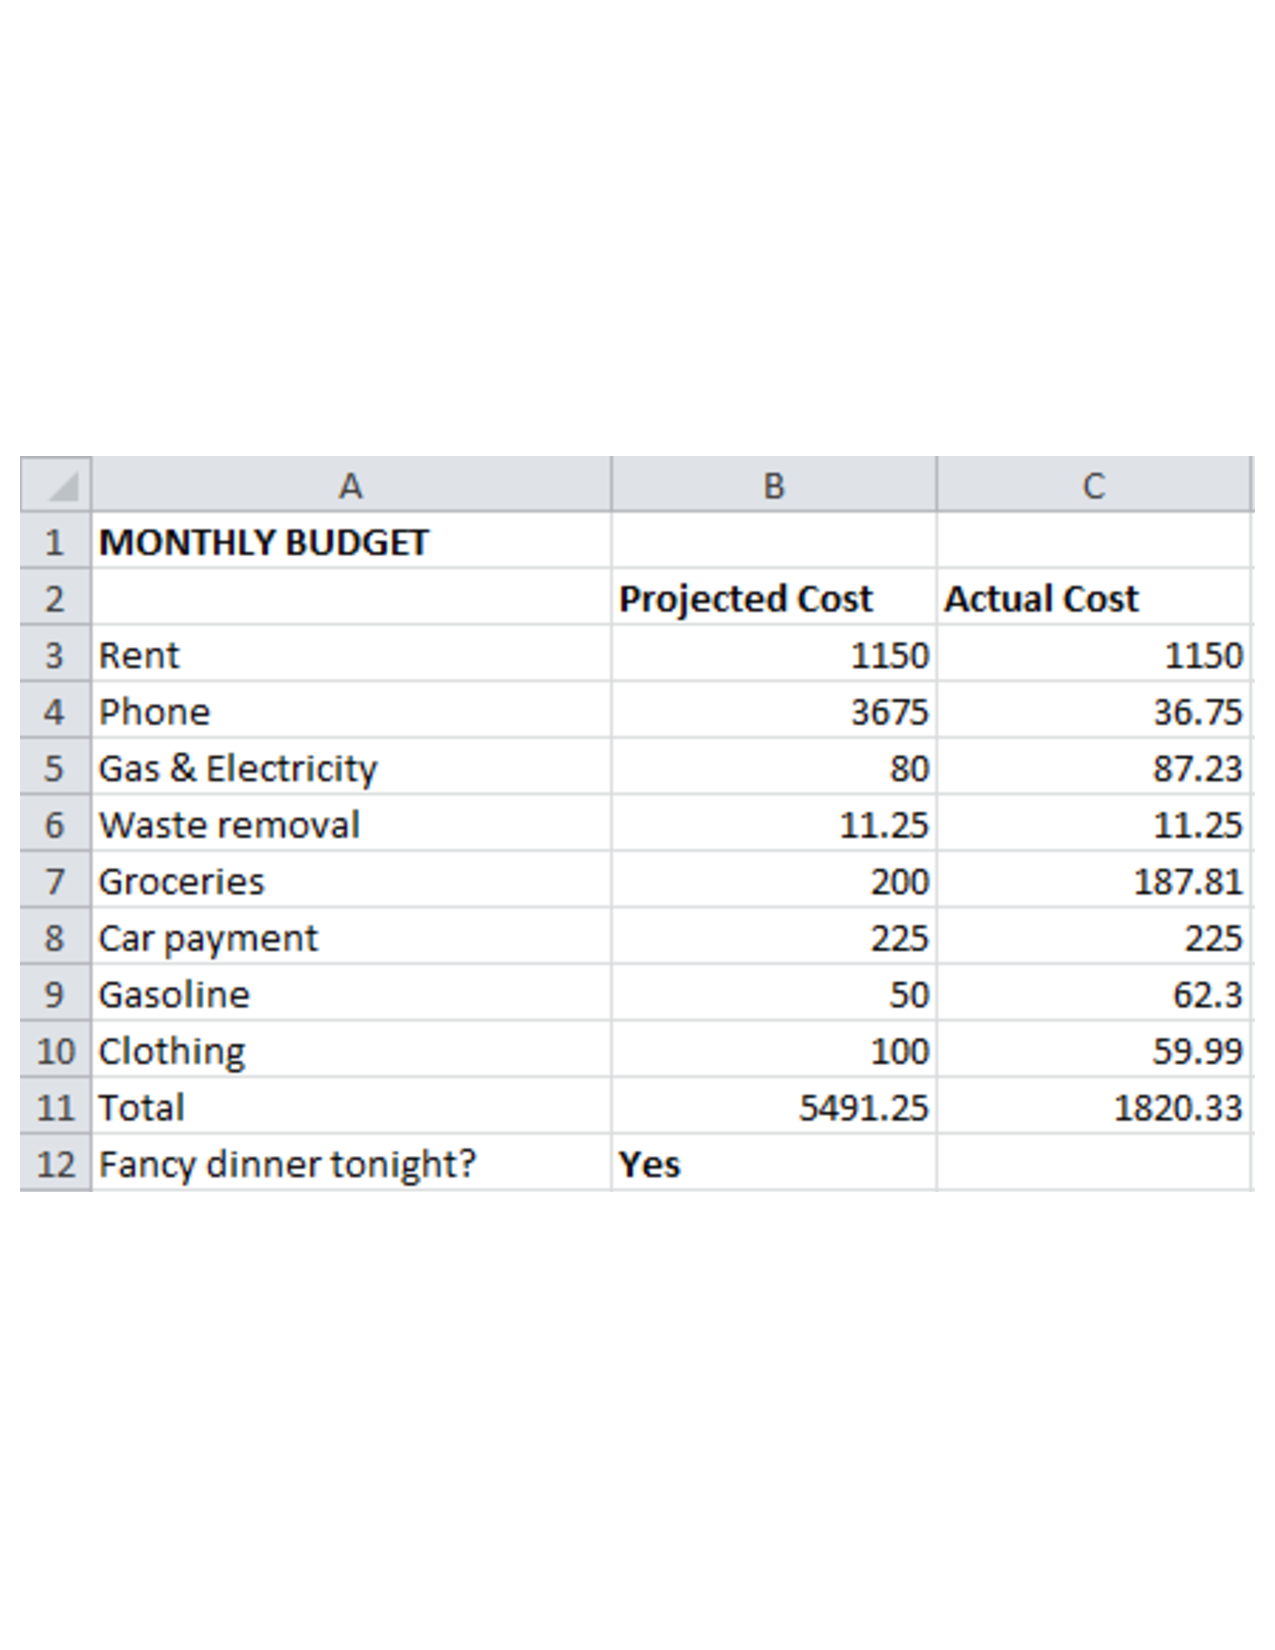
\includegraphics[width=3in]{overview-example}
  \caption{A sample spreadsheet showing a personal budget, with an unfortunate typographical error (see Section~\ref{sec:overview}).\label{fig:personal_budget}}
\end{figure}

\punt{
\begin{table}[t!]
  \centering
    \begin{tabular}{|c|r|r|r|}
    \hline
    & \myalign{c|}{\textsf{\bf{A}}} & \myalign{c|}{\textsf{\bf{B}}} & \myalign{c|}{\textsf{\bf{C}}} \\
    \hline
    \textsf{\textsf{\bf{1}}} & \textsf{MONTHLY BUDGET} & \textsf{Projected Cost} & \textsf{Actual Cost} \\
    \hline
    \textsf{\textsf{\bf{2}}} & \textsf{Rent} & \textsf{\$1150}  & \textsf{\$1150} \\
    \hline
    \textsf{\textsf{\bf{3}}} & \textsf{Phone} & \textsf{\$3675}  & \textsf{\$36.75} \\
    \hline
    \textsf{\textsf{\bf{4}}} & \textsf{Gas} \& \textsf{Electricity} & \textsf{\$80}    & \textsf{\$87.23} \\
    \hline
    \textsf{\textsf{\bf{5}}} & \textsf{Waste removal} & \textsf{\$11.25} & \textsf{\$11.25} \\
    \hline
    \textsf{\textsf{\bf{6}}} & \textsf{Groceries} & \textsf{\$200}   & \textsf{\$187.81} \\
    \hline
    \textsf{\textsf{\bf{7}}} & \textsf{Car payment} & \textsf{\$225}   & \textsf{\$225} \\
    \hline
    \textsf{\textsf{\bf{8}}} & \textsf{Gasoline} & \textsf{\$50}    & \textsf{\$62.3} \\
    \hline
    \textsf{\textsf{\bf{9}}} & \textsf{Clothing} & \textsf{\$100}   & \textsf{\$59.99} \\
    \hline
    \textsf{\textsf{\bf{10}}} & \textsf{Total} & \textsf{\$5491.25} & \textsf{\$1820.33} \\
    \hline
    \textsf{\textsf{\bf{11}}} & \textsf{Fancy dinner tonight?} & \textsf{Yes}   &  \\
    \hline
    \end{tabular}%
  \caption{A sample spreadsheet showing a personal budget, with an unfortunate typographical error.\label{tab:personal_budget}}
\end{table}%
}

This section provides an overview of how data debugging
works. Section~\ref{sec:algorithm} describes the algorithms in full
detail, and Section~\ref{sec:analysis} includes formal analysis of various
aspects of data debugging, including asymptotic performance and
statistical effectiveness.

% in cell \texttt{B3}

% the EUSES repository~\cite{Fisher:2005:ESC:1082983.1083242}

Throughout this section, we use a running example of a budget adapted
from a sample template included with Excel, shown in
Figure~\ref{fig:personal_budget}. This spreadsheet tracks expected
versus real spending on monthly expenses. The spreadsheet indicates
whether the user can afford to splurge and go out to a fancy
restaurant, which is when real spending is at least \$150 less than
expected. However, this example contains an unfortunate typographical
error that could lead the user to spend money that he or she does not
actually have. Note that this spreadsheet has been substantially
reduced from the original, so that finding this error manually in the
original spreadsheet would be substantially more difficult.

\paragraph{Dependence Analysis.}
The first step in data debugging is to identify the relationship of
data (inputs) to computations (outputs). For example, in a database
management system, data inputs would be tuples (records) and computations would
be queries. In a spreadsheet, inputs are data in cells, while
computations are either charts or formulas that are not used by other formulas.

\begin{figure}[!t]
\centering
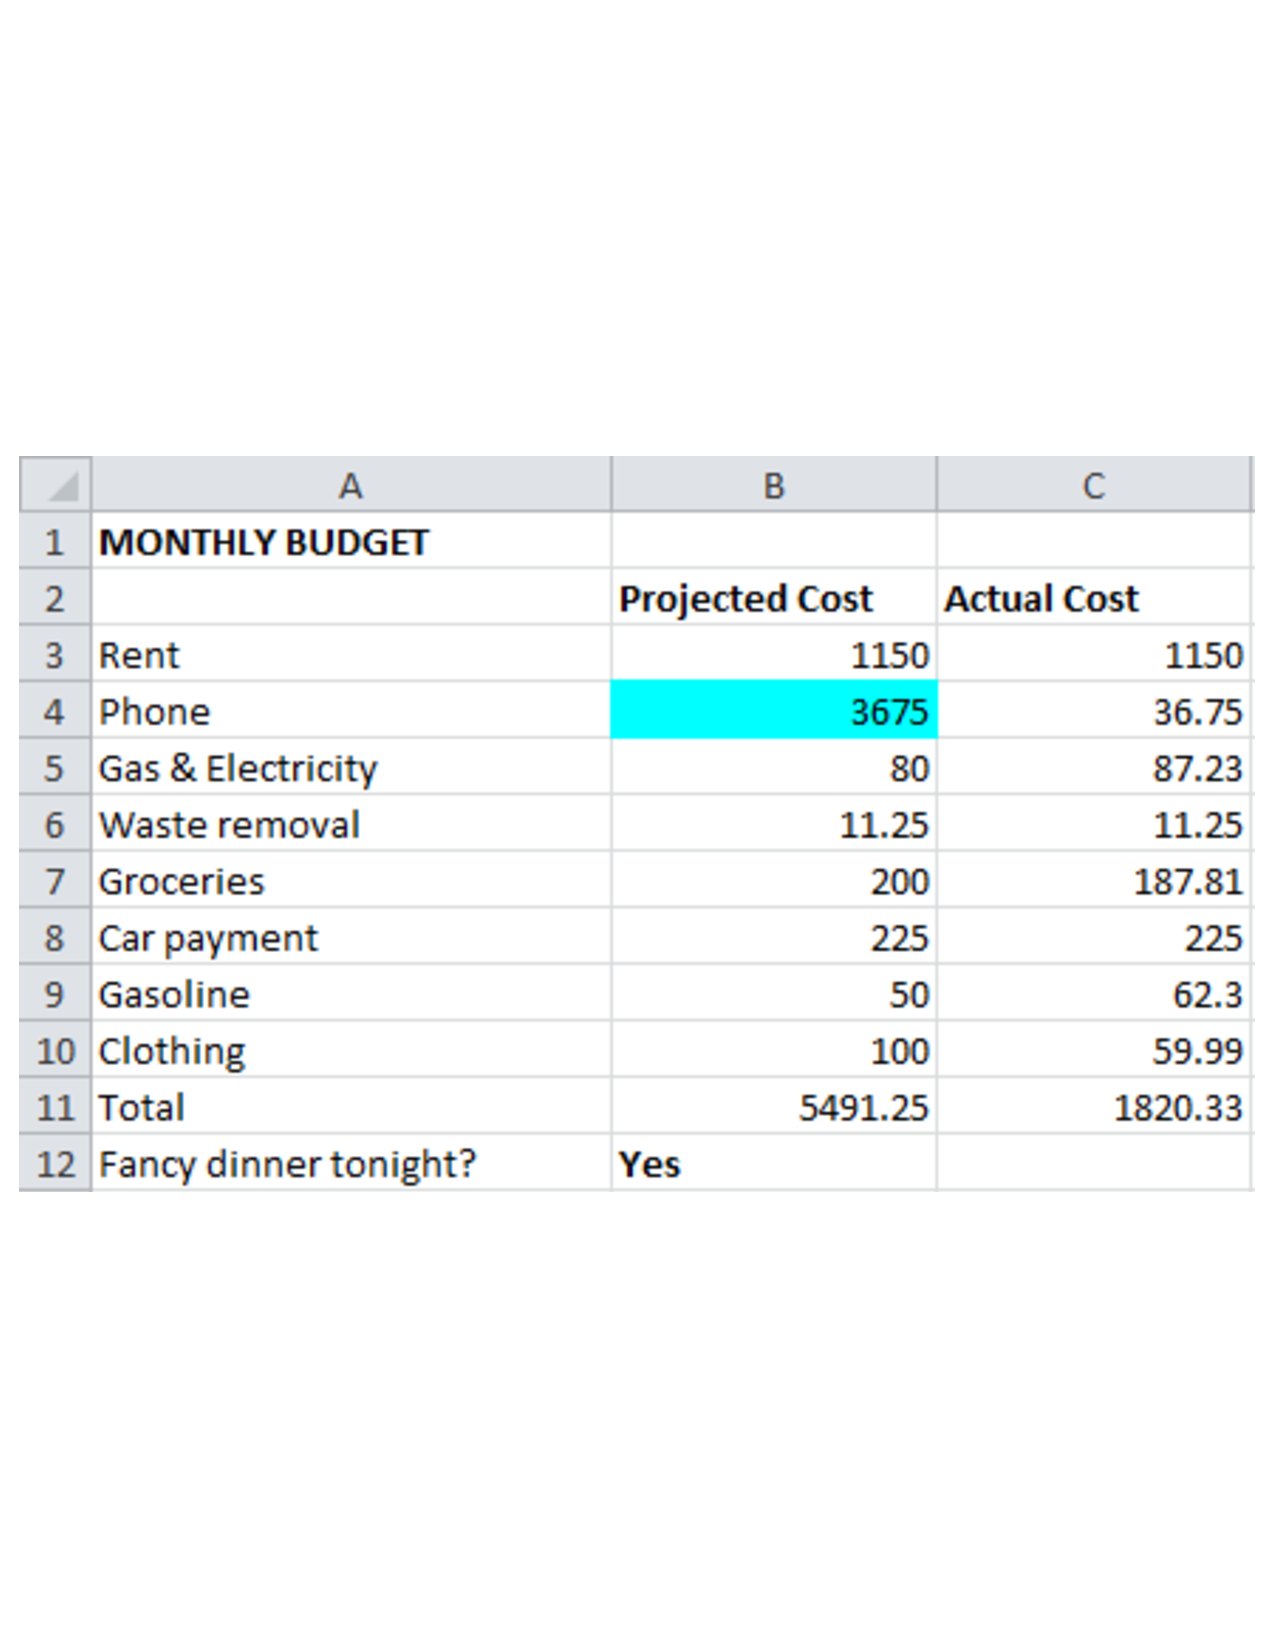
\includegraphics[width=3in]{overview-example-highlighted}
  \caption{The same spreadsheet, with the error highlighted by \checkcell{} as the value with the most impact on the computation.\label{fig:personal_budget_highlighted}}
\end{figure}

\begin{figure}[!b]
\centering
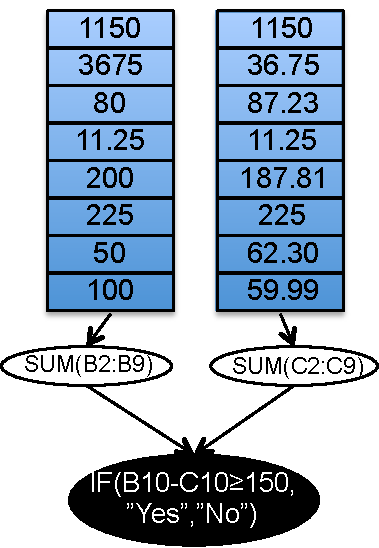
\includegraphics[width=1.75in]{dependence-graph}
\caption{The dependence graph that \checkcell{} extracts from the spreadsheet in Figure~\ref{fig:personal_budget}.\label{fig:dependence-graph}}
\end{figure}
 
Figure~\ref{fig:dependence-graph} shows the dependence graph that \checkcell{}
extracts from this spreadsheet. The final formula, the only output in
this spreadsheet (shown in black), depends on two formulas, which depend on two
disjoint data ranges.


\paragraph{Impact Analysis.}
The next step is to iterate through the data itself to test the impact
of each data item on all computations. For each item, data debugging
repeatedly chooses a random other item from the same ``distribution'',
e.g., another tuple in the same table, or another cell in the same
range, and replaces the item being tested with the randomly-selected
one.

The computations are then recalculated using this new dataset. Changes
in the computations are recorded as their \emph{impact scores} on each
data item.  The impact score for a computation depends on whether the
output is numeric or non-numeric. For numeric data, the impact score
is the normalized change to the original value.
For non-numeric data, the impact score is an \emph{indicator value}: 1
if the result of the computation changed, and 0 if not.

For the spreadsheet in Figure~\ref{fig:personal_budget}, \checkcell{}
starts with cell \texttt{B2}. It chooses a random item from the same
range, for example, cell \texttt{B5}. Replacing \texttt{B2}
with \texttt{B5} results in a new sum, \$4352.50. Since this sum does
not change the \texttt{Yes} answer in the formula, the impact score
for cell \texttt{B2} remains 0.

However, the same procedure for cell \texttt{B3} is likely to have a
different effect.  For example, replacing \texttt{B3}
with \texttt{B8} yields a sum of \$1866.25. The difference
between this sum and actual spending has now dropped below \$150,
triggering a change in the result to \texttt{No}. \checkcell{} then
adds 1 to cell \texttt{B3}'s impact score.

% Each data item maintains a separate impact score for every computation.

To ensure a high degree of statistical confidence in the impact score,
this process is repeated a fixed number of times (at least 30),
accumulating the impact scores associated with each datum. The impact
score is then divided by the number of iterations, resulting in an
average absolute deviation for each data item's impact.

\paragraph{Impact Scoring.}
Finally, the impacts of each data item are normalized by transforming
them into absolute z-scores, where $|z|$ is the absolute distance of
each item from the sample mean, divided by the sample standard
deviation. This \emph{normalized impact score} represents the distance
from the mean impact, in numbers of standard deviations. A standard
approach, which we adopt here, is to only report data whose impact is
at least two standard deviations away from the mean, corresponding to
more than a 95\% level of confidence that these are outliers.  Note
that this interpretation does not depend on normality assumptions
about the data or its impact; in fact, using the normal distribution
to discover anomalous impacts is conservative, as
Section~\ref{sec:analysis} explains.

Each data item's non-zero absolute z-scores are then averaged across
all the outputs, and data debugging assigns that average as the
\emph{overall impact score} of each data item. Intuitively, data with
large overall impact scores either have an extremely high impact on a
small number of computations, or a high impact on many
computations. The overall impact score is used both for ranking and
for displaying the relative anomalousness of the impact of particular
data items, e.g., by coloring such values in brighter colors
corresponding to their distance from the mean.

Figure~\ref{fig:personal_budget_highlighted} shows the effect of
running \checkcell{}, which identifies cell \texttt{B3} as the one
that has the most impact on the spreadsheet.

% ``score'' the impact by highlighting the values proportional to their z-score

% we just need to report outliers in the impact. assuming the impacts
% are normal is a conservative approach: the normal has 0 skewness
% (skew = distribution around the mean -- normal is symmetric, so 0
% skew) and low (either 0 or 3) kurtosis, depending on your definition
% of kurtosis. Every non-normal distribution is by definition more skewed and most
% distributions have a higher kurtosis (heavier tails), so we may
% overmark outliers. We won't find outliers in distributions with
% negative kurtosis, but those are super weird (no tails -- they drop
% below the x-axis at some point on either side), so it's hard to
% argue that they have outliers at all.

